% Options for packages loaded elsewhere
\PassOptionsToPackage{unicode}{hyperref}
\PassOptionsToPackage{hyphens}{url}
%
\documentclass[
  ignorenonframetext,
  aspectratio=169]{beamer}
\usepackage{pgfpages}
\setbeamertemplate{caption}[numbered]
\setbeamertemplate{caption label separator}{: }
\setbeamercolor{caption name}{fg=normal text.fg}
\beamertemplatenavigationsymbolsempty
% Prevent slide breaks in the middle of a paragraph
\widowpenalties 1 10000
\raggedbottom
\setbeamertemplate{part page}{
  \centering
  \begin{beamercolorbox}[sep=16pt,center]{part title}
    \usebeamerfont{part title}\insertpart\par
  \end{beamercolorbox}
}
\setbeamertemplate{section page}{
  \centering
  \begin{beamercolorbox}[sep=12pt,center]{part title}
    \usebeamerfont{section title}\insertsection\par
  \end{beamercolorbox}
}
\setbeamertemplate{subsection page}{
  \centering
  \begin{beamercolorbox}[sep=8pt,center]{part title}
    \usebeamerfont{subsection title}\insertsubsection\par
  \end{beamercolorbox}
}
\AtBeginPart{
  \frame{\partpage}
}
\AtBeginSection{
  \ifbibliography
  \else
    \frame{\sectionpage}
  \fi
}
\AtBeginSubsection{
  \frame{\subsectionpage}
}
\usepackage{amsmath,amssymb}
\usepackage{iftex}
\ifPDFTeX
  \usepackage[T1]{fontenc}
  \usepackage[utf8]{inputenc}
  \usepackage{textcomp} % provide euro and other symbols
\else % if luatex or xetex
  \usepackage{unicode-math} % this also loads fontspec
  \defaultfontfeatures{Scale=MatchLowercase}
  \defaultfontfeatures[\rmfamily]{Ligatures=TeX,Scale=1}
\fi
\usepackage{lmodern}
\ifPDFTeX\else
  % xetex/luatex font selection
\fi
% Use upquote if available, for straight quotes in verbatim environments
\IfFileExists{upquote.sty}{\usepackage{upquote}}{}
\IfFileExists{microtype.sty}{% use microtype if available
  \usepackage[]{microtype}
  \UseMicrotypeSet[protrusion]{basicmath} % disable protrusion for tt fonts
}{}
\makeatletter
\@ifundefined{KOMAClassName}{% if non-KOMA class
  \IfFileExists{parskip.sty}{%
    \usepackage{parskip}
  }{% else
    \setlength{\parindent}{0pt}
    \setlength{\parskip}{6pt plus 2pt minus 1pt}}
}{% if KOMA class
  \KOMAoptions{parskip=half}}
\makeatother
\usepackage{xcolor}
\newif\ifbibliography
\usepackage{listings}
\newcommand{\passthrough}[1]{#1}
\lstset{defaultdialect=[5.3]Lua}
\lstset{defaultdialect=[x86masm]Assembler}
\setlength{\emergencystretch}{3em} % prevent overfull lines
\providecommand{\tightlist}{%
  \setlength{\itemsep}{0pt}\setlength{\parskip}{0pt}}
\setcounter{secnumdepth}{-\maxdimen} % remove section numbering
\setbeamersize{text margin left=0.35cm}
\setbeamersize{text margin right=0.35cm}

\definecolor{peach}{HTML}{EDD1B0}
\setbeamercolor{background canvas}{bg=peach}


\let\oldverbatim\verbatim
\let\oldendverbatim\endverbatim
\renewenvironment{verbatim}{\scriptsize\oldverbatim}{\oldendverbatim}

% \renewenvironment{Shaded}{\begin{snugshade}\footnotesize}{\end{snugshade}}

\setbeamertemplate{itemize item}{>}
\setbeamertemplate{itemize subitem}{--}

\setbeamerfont{itemize/enumerate body}{size=\large}
\setbeamerfont{itemize/enumerate subbody}{size=\large}
\setbeamerfont{itemize/enumerate subsubbody}{size=\small}

\setbeamerfont{normal text}{size=\tiny}

\usepackage{listings}
\lstset{basicstyle=\small}

\setbeamertemplate{footline}[page number]
\ifLuaTeX
  \usepackage{selnolig}  % disable illegal ligatures
\fi
\usepackage{bookmark}
\IfFileExists{xurl.sty}{\usepackage{xurl}}{} % add URL line breaks if available
\urlstyle{same}
\hypersetup{
  pdftitle={Elixir\textquotesingle s Set-Theoretic Type System},
  pdfauthor={Robert Ellen},
  hidelinks,
  pdfcreator={LaTeX via pandoc}}

\title{Elixir\textquotesingle s Set-Theoretic Type System}
\author{Robert Ellen}
\date{2024/11/12}

\begin{document}
\frame{\titlepage}

\section{Summary}\label{summary}

\section{Elixir}\label{elixir-1}

\begin{frame}{Elixir}


\end{frame}

\begin{frame}{What is the Erlang Ecosystem?}
\phantomsection\label{what-is-the-erlang-ecosystem}
A group of languages, libraries, frameworks, and applications that are
implemented on top of the Erlang virtual machine, the BEAM.

Languages include:

\begin{figure}
\centering
\begin{minipage}{.24\textwidth}
  \centering
  
\includegraphics[width=.8\linewidth]{./img/erlang_logo.png}
\end{minipage}
\begin{minipage}{.24\textwidth}
  \centering
  
\includegraphics[width=.8\linewidth]{./img/elixir-vertical.png}
\end{minipage}
\begin{minipage}{.24\textwidth}
  \centering
  
\includegraphics[width=.8\linewidth]{./img/lucy.png}
\end{minipage}
\begin{minipage}{.24\textwidth}
  \centering
  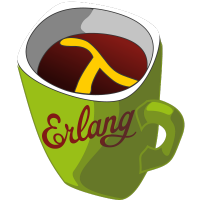
\includegraphics[width=.8\linewidth]{./img/lfe.png}
\end{minipage}
\end{figure}

\ldots plus dozens more
\end{frame}

\begin{frame}{What is the Erlang Ecosystem?}
\phantomsection\label{what-is-the-erlang-ecosystem-1}
Libraries and frameworks include:

\begin{figure}
\centering
\begin{minipage}{.24\textwidth}
  \centering
 \LARGE{OTP}
\end{minipage}
\begin{minipage}{.24\textwidth}
  \centering
  
\includegraphics[width=.8\linewidth]{./img/rabbitmq_logo.png}
\end{minipage}
\begin{minipage}{.24\textwidth}
  \centering
  
\includegraphics[width=.8\linewidth]{./img/phoenix_logo.png}
\end{minipage}
\begin{minipage}{.24\textwidth}
  \centering
  
\includegraphics[width=.8\linewidth]{./img/ecto_logo.png}
\end{minipage}
\begin{minipage}{.24\textwidth}
\centering
  
\includegraphics[width=.8\linewidth]{./img/absinthe_logo.png}
\end{minipage}
\begin{minipage}{.24\textwidth}
\centering
  
\includegraphics[width=.8\linewidth]{./img/oban-logo.png}
\end{minipage}
\begin{minipage}{.24\textwidth}
  \centering
  
\includegraphics[width=.7\linewidth]{./img/nx_logo.png}
\end{minipage}
\begin{minipage}{.24\textwidth}
  \centering
  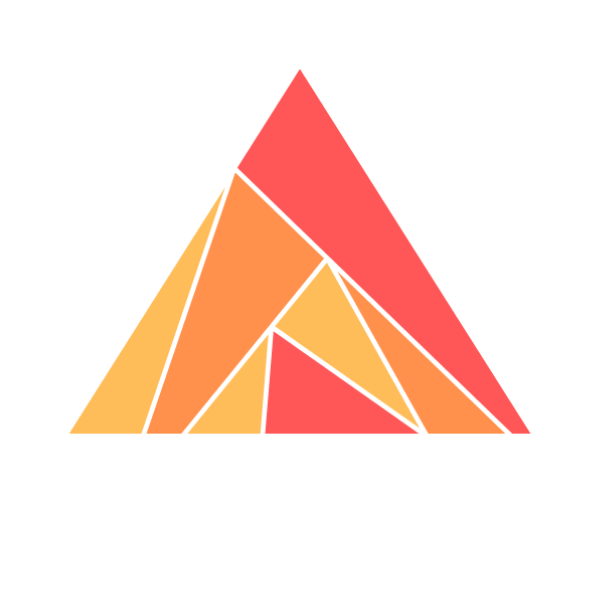
\includegraphics[width=.8\linewidth]{./img/ash-logo.png}
\end{minipage}
\end{figure}
\end{frame}

\begin{frame}{What is the Erlang Ecosystem?}
\phantomsection\label{what-is-the-erlang-ecosystem-2}
Built around a shared value in:

\begin{itemize}
\tightlist
\item
  massive concurrency
\item
  fault-tolerance
\item
  simplicity
\item
  acknowledging the errors will occur so lets deal with them

  \begin{itemize}
  \tightlist
  \item
    ``Let it crash"--have a plan to restart sub-systems when they crash
  \end{itemize}
\end{itemize}
\end{frame}

\begin{frame}{Brief history of Erlang}
\phantomsection\label{brief-history-of-erlang}
\centering
covered in my 2013 talk, but tonight...
\end{frame}

\begin{frame}{Brief history of Erlang}
\phantomsection\label{brief-history-of-erlang-1}
\begin{center}

\includegraphics[width=.5\textwidth]{./img/short_short.jpg}
\end{center}
\end{frame}

\begin{frame}{Brief history of Erlang}
\phantomsection\label{brief-history-of-erlang-2}
\begin{itemize}
\tightlist
\item
  developed in the mid 1980s at Ericsson
\item
  to run on next generation telephone switches

  \begin{itemize}
  \tightlist
  \item
    concurrent, fault-tolerant, distributed, soft real-time
  \item
    reports of 1200k LOC and ``nine nines" of uptime on the AXD301
    switch
  \item
    reports of market penetration of \textgreater{} 50\% in mobile
    telephony switches
  \end{itemize}
\item
  solved web-scale in the \textquotesingle80s
\end{itemize}

\begin{figure}
\centering
\begin{minipage}{.24\textwidth}
  \centering
  
\includegraphics[width=.9\linewidth]{./img/joe.jpg}
\end{minipage}
\begin{minipage}{.24\textwidth}
  \centering
  
\includegraphics[width=.9\linewidth]{./img/mike.jpeg}
\end{minipage}
\begin{minipage}{.24\textwidth}
  \centering
  
\includegraphics[width=.9\linewidth]{./img/robert.jpeg}
\end{minipage}
\begin{minipage}{.24\textwidth}
  \centering
  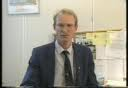
\includegraphics[width=.9\linewidth]{./img/bjarne.jpg}
\end{minipage}
\end{figure}
\end{frame}

\begin{frame}{The BEAM}
\phantomsection\label{the-beam}
\begin{itemize}
\tightlist
\item
  Erlang\textquotesingle s virtual machine / runtime system
\item
  lightweight processes, SMP
\item
  multi-generational, per-process garbage collector
\item
  asynchronous, location-transparent, message-passing IPC
\item
  hot-code-loading
\item
  powerful REPL and introspection tools
\item
  new JIT compiler (BEAM bytecode to machine code)
\end{itemize}
\end{frame}

\begin{frame}[fragile]{The OTP libraries}
\phantomsection\label{the-otp-libraries}
\begin{itemize}
\tightlist
\item
  Erlang\textquotesingle s "standard library"
\item
  dozens of modules providing various typical stdlib stuff
\item
  core of which are for supervision trees

  \begin{itemize}
  \tightlist
  \item
    \passthrough{\lstinline!gen\_server!} - actors / workers
  \item
    supervisors - handling starting/stopping/restarting
    \passthrough{\lstinline!gen\_servers!}
  \end{itemize}
\end{itemize}
\end{frame}

\begin{frame}{supervision trees}
\phantomsection\label{supervision-trees}
\begin{center}
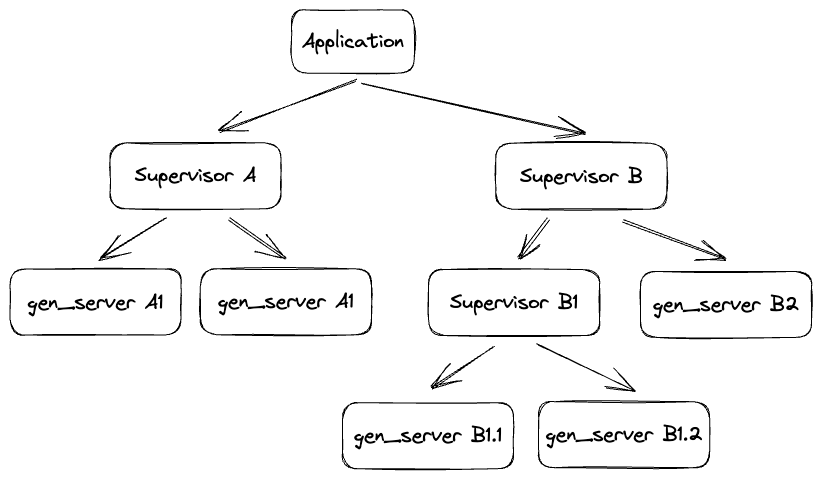
\includegraphics[width=0.8\textwidth]{./img/tree.png}
\end{center}
\end{frame}

\begin{frame}{Elixir}
\phantomsection\label{elixir}
There will be some comparing and contrasting of Gleam with
Elixir\ldots{}

\begin{center}

\includegraphics[width=.5\textwidth]{./img/elixir_logo.png}
\end{center}
\end{frame}

\begin{frame}{Brief history of Elixir}
\phantomsection\label{brief-history-of-elixir}
\begin{itemize}
\tightlist
\item
  created by José Valim starting in 2012
\item
  inspired by Erlang, Ruby, and, to a lesser extent, Lisp
\item
  like Erlang, the language is quite stable
\end{itemize}

\begin{center}

\includegraphics[width=.5\textwidth]{./img/elixir_logo.png}
\end{center}
\end{frame}

\begin{frame}[fragile]{Features of Elixir}
\phantomsection\label{features-of-elixir}
\begin{itemize}
\tightlist
\item
  Ruby-like syntax while retaining most of Erlang\textquotesingle s
  semantics

  \begin{itemize}
  \tightlist
  \item
    \ldots, immutable data, HoF, side-effects anywhere,
    dynamically-typed, \ldots{}
  \end{itemize}
\item
  interoperate with Erlang
\item
  hygienic macros
\item
  highly ergonomic build tool: \passthrough{\lstinline!mix!}
\item
  modern package manager: \passthrough{\lstinline!hex!}
\item
  excellent unit test tool: exunit
\item
  opinionated formatter
\item
  drops strict SSA in favour of rebinding
\end{itemize}
\end{frame}

\section{Typing BEAM languages}\label{typing-beam-languages}

\begin{frame}{Marlow \& Wadler - 1997}
\phantomsection\label{marlow-wadler---1997}
\begin{itemize}
\tightlist
\item
  ``We can stop waiting for functional languages to be used in
  practice--that day is here!"
\item
  threw away Hindley-Milner: \(U = V\) -- this would not work with
  existing Erlang codebases
\item
  proposed strictly more general sub-typing instead: \(U \subseteq V\)
\end{itemize}
\end{frame}

\begin{frame}{eqWAlizer}
\phantomsection\label{eqwalizer}
Developed by Meta for WhatsApp
\end{frame}

\begin{frame}{Typed BEAM languages with alternate semantics}
\phantomsection\label{typed-beam-languages-with-alternate-semantics}
\begin{itemize}
\tightlist
\item
  Hamler - purescript for the BEAM
\item
  Caramel - ML for the BEAM
\item
  Gleam - HM-based type system - see my May 2024 talk
\item
  \ldots{}
\end{itemize}
\end{frame}

\begin{frame}{Static analysis tools}
\phantomsection\label{static-analysis-tools}
\begin{itemize}
\tightlist
\item
  dialyzer - Linhahl \& Sagonas, 2006
\item
  gradualizer
\end{itemize}
\end{frame}

\section{References}\label{references}

\begin{frame}{References}
Simon Marlow and Philip Wadler. A practical subtyping system for erlang.
In Proceedings of the Second ACM SIGPLAN International Conference on
Functional Programming, ICFP '97, page 136--149, New York, NY, USA,
1997. Association for Computing Machinery.
\url{doi:10.1145/258948.258962}.

Tobias Lindahl and Konstantinos Sagonas. Practical type inference based
on success typings. In ACM-SIGPLAN International Conference on
Principles and Practice of Declarative Programming, 2006.
\url{doi:10.1145/1140335.1140356}.
\end{frame}

\begin{frame}{Thank you}
\phantomsection\label{thank-you}
I\textquotesingle ll post slides soon.
\end{frame}

\end{document}
